\section{Análisis de los resultados obtenidos}\label{error_analysis}
% resultados experimentos
A partir de las hipótesis planteadas es posible dar cuenta de que a veces los resultados esperados según la teoría no se dan en la práctica, y que en algunos casos puede resultar mejor entrenar una arquitectura propia desde cero que intentar sacar provecho de redes preentrenadas. Como se pudo observar en el trabajo, ninguno de los experimentos que se hicieron utilizando aprendizaje mediante transferencia alcanzó los resultados obtenidos por la arquitectura planteada en el experimento \ref{sssec:exp2} para el conjunto de datos de \cite{vision_based_real_estate_price_estimation}.

% análisis del error mejores dos redes (exp 2 y exp 6)
\subsection{Error por categoría modelos obtenidos en los experimentos \ref{sssec:exp2} y \ref{sssec:exp6}}
Como se observa en las tablas \ref{conclusiones:error_analysis:exp2} y \ref{conclusiones:error_analysis:exp6}, no todas las categorías se predicen correctamente en la misma medida, es decir, cada modelo aprende a clasificar mejor algunas categorías que otras. Llama la atención que para estos modelos se cumple que el orden de las categorías contabilizando clasificaciones incorrectas es el mismo en ambos, es decir, ambos modelos tienen menor cantidad de errores en las mismas categorías; el orden (ascendente) es: \(frontyard\), \(bathroom\), \(dining room\), \(kitchen\), \(bedroom\) y \(livingRoom\). Tanto la calidad de las imágenes de las categorías con mayor tasa de error como el solapamiento de posibles entidades que pueden formar parte de estas escenas son razones que podrían explicar este comportamiento. 


\begin{table}[h!]
	\centering
	\begin{tabular}{| l | r | r |}
		\toprule
		Categoría &    Cantidad errores &     \% del total \\
		\midrule
		frontyard &  100 &  0.06 \\
		bathroom &  182 &  0.11 \\
		dining\_room &  220 &  0.13 \\
		kitchen &  269 &  0.16 \\
		bedroom &  384 &  0.23 \\
		livingRoom &  497 &  0.30 \\
		\bottomrule
	\end{tabular}
	\caption{Error por categoría y porcentaje sobre el total - Modelo del experimento \ref{sssec:exp2}}
	\label{conclusiones:error_analysis:exp2}
\end{table}

\begin{table}[h!]
	\centering
	\begin{tabular}{| l | r | r |}
		\toprule
		Categoría &    Cantidad errores &     \% del total \\
		\midrule
		frontyard &  145 &  0.06 \\
		bathroom &  148 &  0.07 \\
		dining\_room &  356 &  0.16 \\
		kitchen &  504 &  0.22 \\
		bedroom &  537 &  0.24 \\
		livingRoom &  574 &  0.25 \\
		\bottomrule
	\end{tabular}
	\caption{Error por categoría y porcentaje sobre el total - Modelo delexperimento \ref{sssec:exp6}}
	\label{conclusiones:error_analysis:exp6}
\end{table}

\subsection{Distribución de probabilidades de salida para clasificaciones erróneas}
% análisis de pred proba en errores
% 	> con qué porcentaje se predice cuando se equivoca en cada categoría? (media de pred proba en errores por categoría)
%	> a qué resultado se llega cuando se setea un umbral mínimo (¿0.4?) para las predicciones? (sklearn.metrics.accuracy tomando sólo los casos en los que pred_proba fue mayor que THRESHOLD -¿0.4?-)
Como se mencionó en \ref{sec:marco_teorico}, la capa de salida de una red con activación \(Softmax\) devuelve la probabilidad de cada clase (de las que luego se elije la de mayor magnitud). 

Una situación que puede estar sucediendo es que en los aquellos casos en que las redes fallan en su clasificación, la magnitud de la probabilidad que arrojan es baja. Una forma de analizar estos casos es mediante algunos estadísticos simples de las probabilidades asignadas a cada clase cuando la red falló. 

A diferencia de lo que se podía esperar, las redes se equivocan prediciendo con probabilidades mayores o iguales a 0.5, lo cual es una probabilidad alta ya que queda el resto (entre 1 y esta probabilidad) para las demás 5 clases. 
   
\begin{table}[h!]
	\centering
	\begin{tabular}{| l | rrrrr| }
		\toprule
		Categoría & \multicolumn{5}{l}{Probabilidad asignada} \\
		&         media & mediana &   desvío &   mín. &   máx. \\
		\midrule
		bathroom &         0.63 &   0.61 &  0.20 &  0.26 &  1.00 \\
		bedroom &         0.64 &   0.62 &  0.18 &  0.26 &  1.00 \\
		dining\_room &         0.67 &   0.64 &  0.19 &  0.26 &  1.00 \\
		frontyard &         0.63 &   0.62 &  0.19 &  0.26 &  0.99 \\
		kitchen &         0.66 &   0.63 &  0.19 &  0.31 &  1.00 \\
		livingRoom &         0.69 &   0.70 &  0.19 &  0.26 &  1.00 \\
		\bottomrule
	\end{tabular}
	\caption{Estadísticos de probabilidades asignadas en clasificaciones erróneas - Modelo delexperimento \ref{sssec:exp2}}
	\label{conclusiones:error_analysis_pred_proba_stats:exp2}
\end{table}

\begin{table}[h!]
	\centering
	\begin{tabular}{| l | rrrrr | }
		\toprule
		Categoría & \multicolumn{5}{l}{Probabilidad asignada} \\
		&         media & mediana &   desvío &   mín. &   máx. \\
		\midrule
		bathroom &         0.56 &   0.53 &  0.19 &  0.19 &  1.00 \\
		bedroom &         0.59 &   0.56 &  0.19 &  0.25 &  1.00 \\
		dining\_room &         0.60 &   0.57 &  0.18 &  0.20 &  1.00 \\
		frontyard &         0.55 &   0.50 &  0.20 &  0.19 &  0.98 \\
		kitchen &         0.61 &   0.59 &  0.19 &  0.23 &  1.00 \\
		livingRoom &         0.61 &   0.59 &  0.19 &  0.22 &  1.00 \\
		\bottomrule
	\end{tabular}
	\caption{Estadísticos de probabilidades asignadas en clasificaciones erróneas - Modelo delexperimento \ref{sssec:exp6}}
	\label{conclusiones:error_analysis_pred_proba_stats:exp6}
\end{table}

Conforme estos resultados se analizan, surge el interrongante de conocer qué sucedería si se define un umbral mínimo para siquiera considerar la predicción de un modelo, es decir que los casos que tengan una probabilidad por debajo del umbral directamente se configuren como no predecibles o no aceptados. En las figuras \ref{fig:resultsexp2errorsbythreshold} y \ref{fig:resultsexp6errorsbythreshold} se puede observar tanto la cantidad de casos alcanzados utilizando diferentes umbrales, la exactitud categórica y el porcentaje de errores que se dejarían de cometer para umbrales entre cero y uno. 

En la figura \ref{fig:resultsexp2errorsbythreshold} con un umbral de 0.55 se alcanzaría a predecir 5480 de los 6328 casos totales con una exactitud categórica del \%80, mientras que utilizando el mismo umbral para el modelo del experimento \ref{sssec:exp6}, en la figura \ref{fig:resultsexp6errorsbythreshold} se alcanzan sólo 4625 casos, con un \%71 de exactitud categórica. 

\begin{figure}[h!]
	\centering
	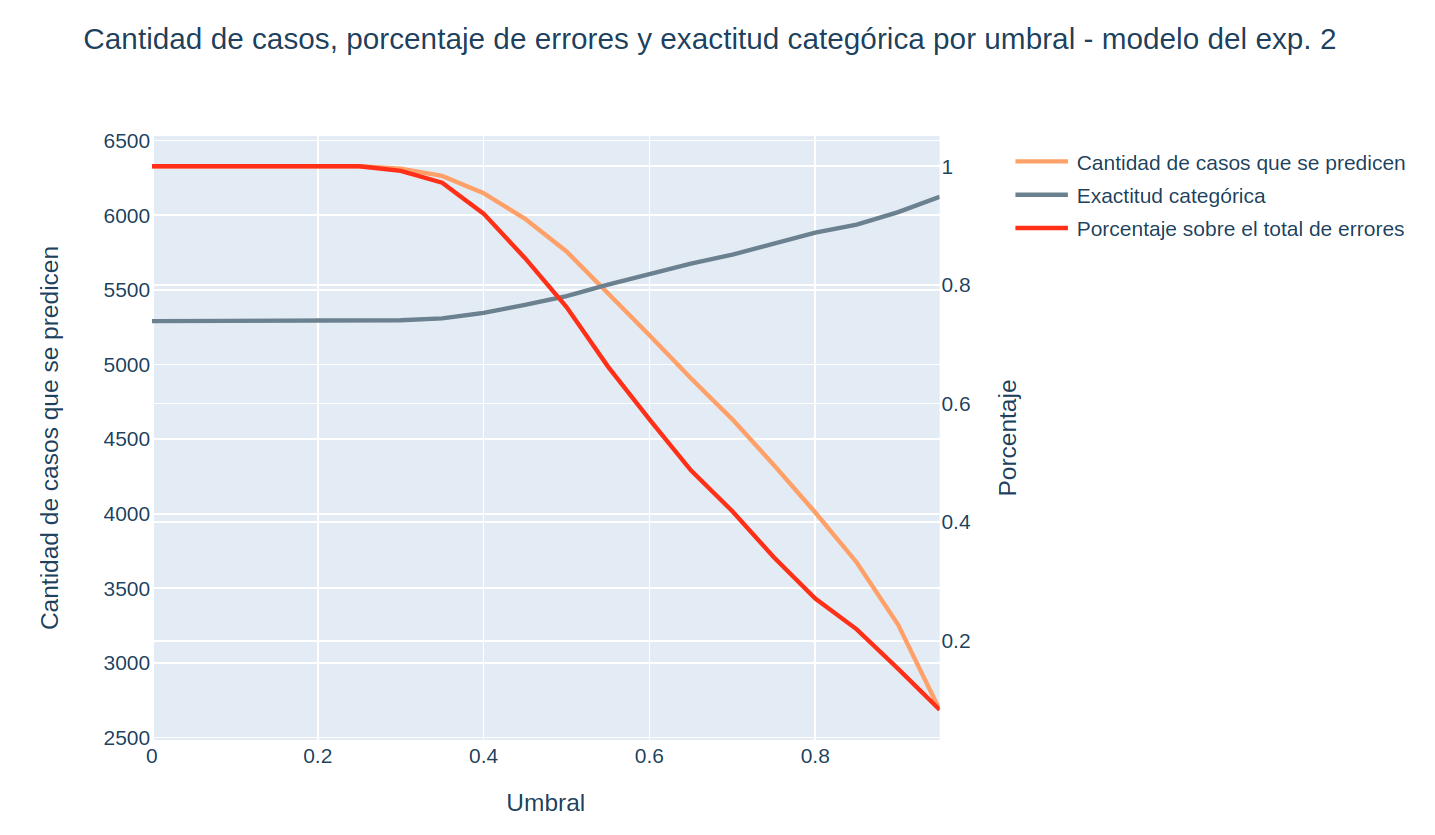
\includegraphics[width=1.1\linewidth]{images/results_exp_2_errors_by_threshold}
	\caption{Cantidad de erorres y exactitud categórica por umbral para el modelo del experimento \ref{sssec:exp2}}
	\label{fig:resultsexp2errorsbythreshold}
\end{figure}

\begin{figure}[h!]
	\centering
	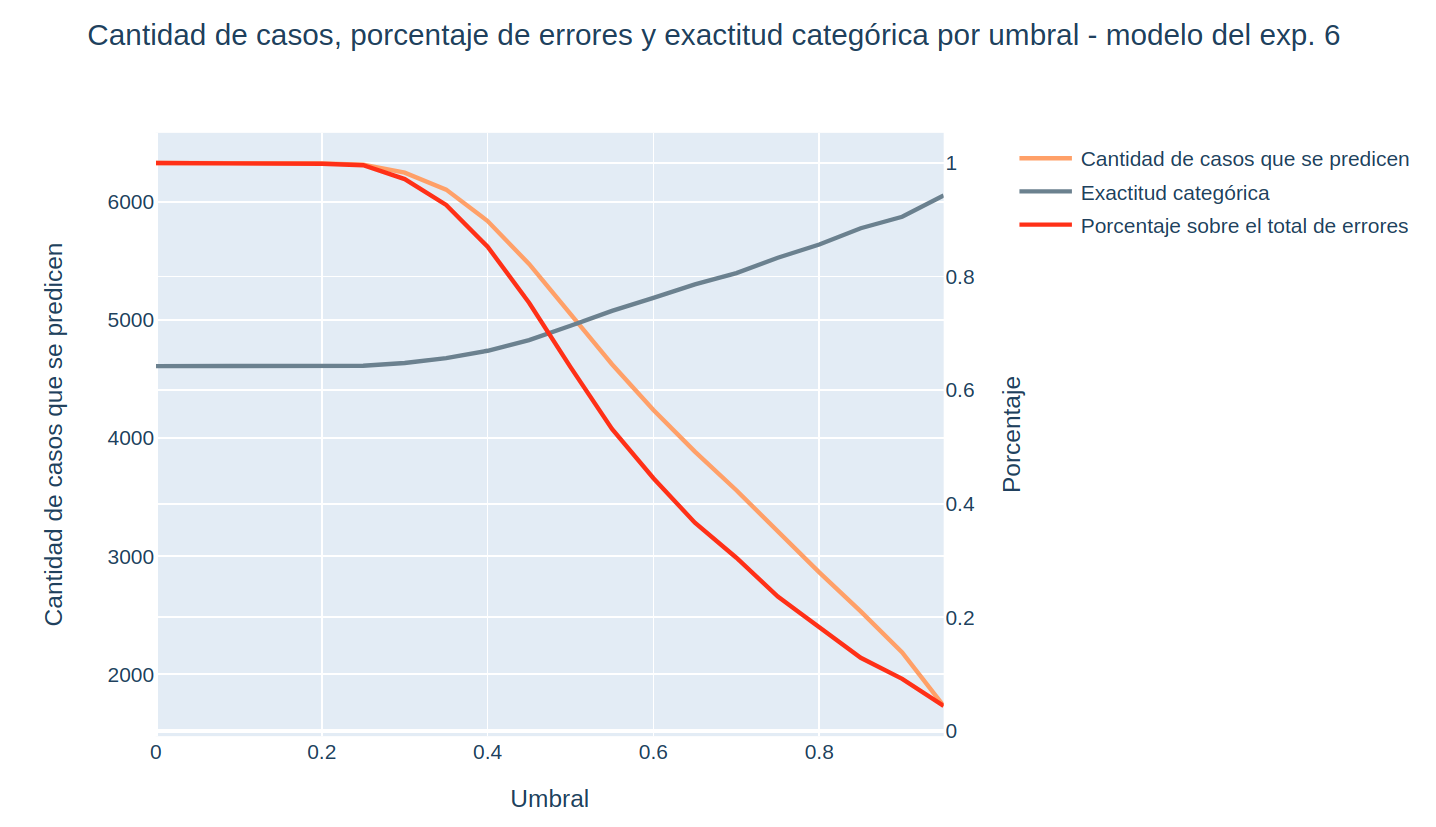
\includegraphics[width=1.1\linewidth]{images/results_exp_6_errors_by_threshold}
	\caption{Cantidad de erorres y exactitud categórica por umbral para el modelo del experimento \ref{sssec:exp6}}
	\label{fig:resultsexp6errorsbythreshold}
\end{figure}

En las figuras \ref{fig:results_exp_2_distribution_of_pred_proba} y \ref{fig:results_exp_6_distribution_of_pred_proba} podemos observar un gráfico de caja de la probabilidad con la que se determinó cada etiqueta, dividido por categoría según si fueron correcta o incorrectamente clasificados. En los mismos podemos observar que para los casos clasificados correctamente las predicciones tienen distribuciones de probabilidad muy diferentes a los casos incorrectos, por lo que cobra mayor sentido seleccionar un umbral para las predicciones. Un punto no menor a mencionar es que la etiqueta \(frontyard\) es la que ambos modelos mejor predicen, mientras que las mayores difrencias entre cada modelo se observan en las categorías \(kitchen\) y \(bathroom\). 

\begin{figure}[h!]
	\centering
	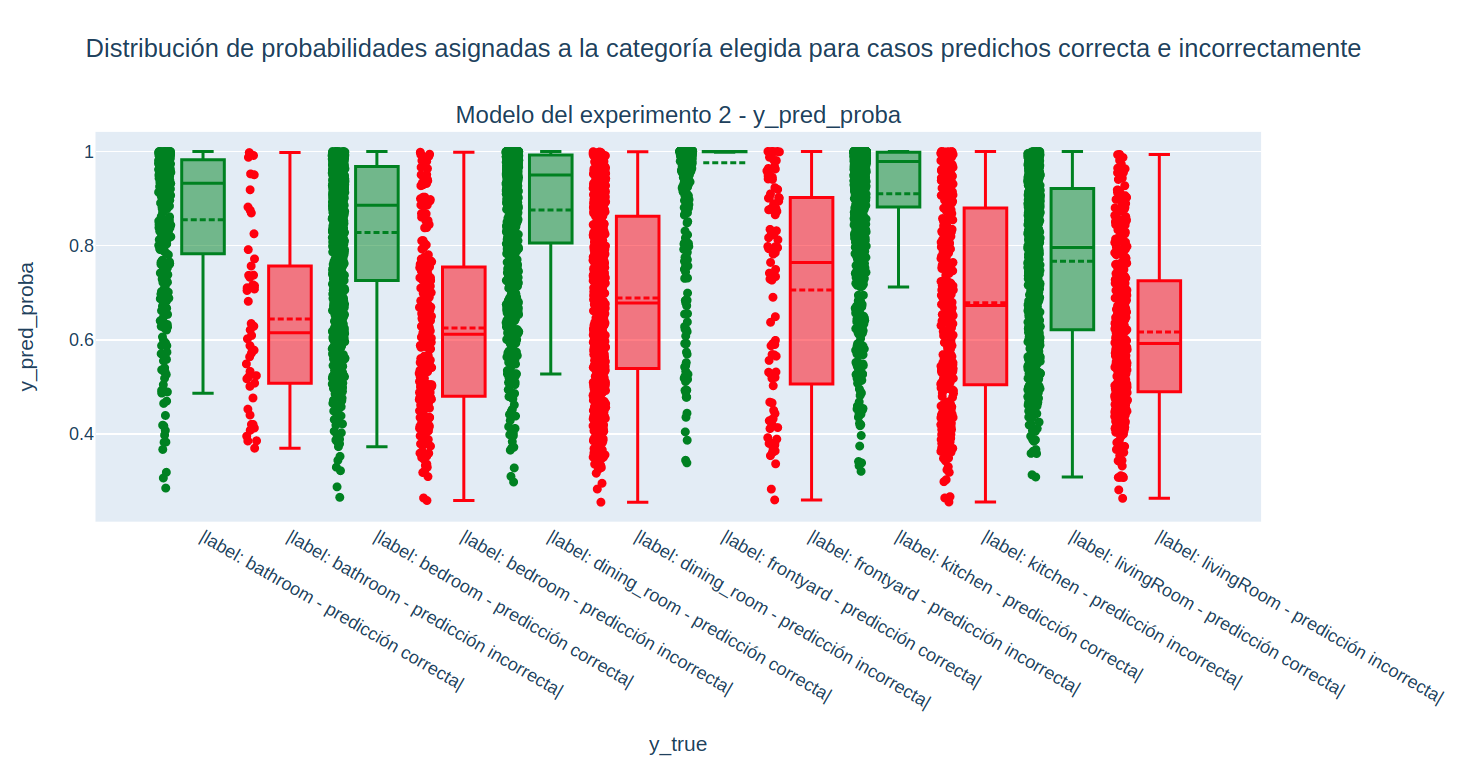
\includegraphics[width=1.1\linewidth]{images/results_exp_2_distribution_of_pred_proba}
	\caption{Distribución de probabilidades asignadas por clase para el modelo del experimento \ref{sssec:exp6}}
	\label{fig:results_exp_2_distribution_of_pred_proba}
\end{figure}

\begin{figure}[h!]
	\centering
	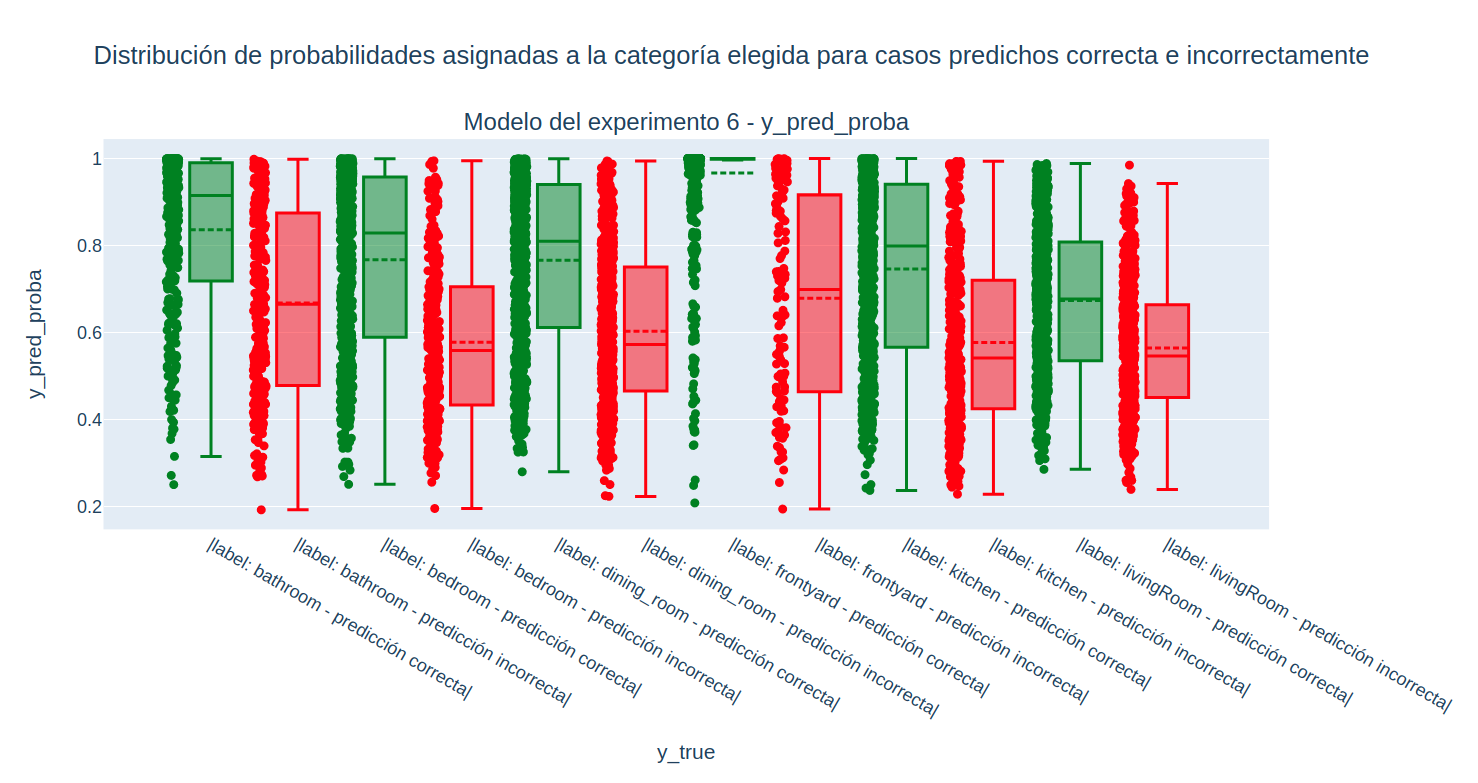
\includegraphics[width=1.1\linewidth]{images/results_exp_6_distribution_of_pred_proba}
	\caption{Distribución de probabilidades asignadas por clase para el modelo del experimento \ref{sssec:exp6}}
	\label{fig:results_exp_6_distribution_of_pred_proba}
\end{figure}


% análisis de casos que deberían ser predecibles por ambas dos mejores redes (exp 2 y exp 7)
\subsection{Exactitud categórica casos que deberían poder predecirse correctamente}
A continuación se revisará un subconjunto de casos que deberían ser clasificados correctamente por un modelo, debido a que son claros ejemplos de la clase a la que se corresponden. Este subconjunto contiene 25 imágenes por categoría seleccionadas del conjunto de verificación utilizado para los experimentos \ref{sssec:exp2} al \ref{sssec:exp6}. 

La tabla \ref{conclusiones:subset:results} muestra que para el subconjunto elegido los modelos obtienen un gran incremento en relación a las métricas proporcionadas anteriormente. Se puede razonar que las imágenes que peor resultado tienen son aquellas que contienen demasiado ruido en relación al relacionado a la escena.

\begin{table}[h!]
	\centering
	\begin{tabular}{| l | r |}
		\toprule
		Modelo obtenido en & Exactitud Categórica \\
		experimento & Subconjunto elegido \\
		\midrule
		Experimento 2 (\ref{sssec:exp2}) & 0.94 \\
		\midrule
		Experimento 6 (\ref{sssec:exp6}) & 0.78 \\
		\bottomrule
	\end{tabular}\caption{Resultados obtenidos por los modelos en experimentos \ref{sssec:exp2} y \ref{sssec:exp6} para el subconjunto de imágenes elegido}
	\label{conclusiones:subset:results}
\end{table}

